%-----------------------------------
%   PROTOCOLOS DE ENRUTAMIENTO
%-----------------------------------
\chapter{Protocolos de enrutamiento}

\label{ch:protocolos_de_enrutamiento}

Los protocolos de enrutamiento se encargan de determinar las rutas que deben
seguir los datagramas para llegar a su destino. En las redes de
infraestructura fija, la topología cambia muy poco, por lo que es raro que las
rutas tengan que modificarse. Sin embargo, en la sección \ref{ch:vanets} vimos
que una de las características de las VANETs es que la topología cambia todo el
tiempo. Esto hace que la vigencia de las rutas sea muy corta, por lo que se
necesitan protocolos de enrutamiento que puedan lidiar con estos problemas.

En este capítulo, se explica cómo se almacenan las rutas y cómo se usan para
retransmitir los datagramas de nodo a nodo. Después, se presentan diferentes
enfoques de enrutamiento para redes descentralizadas, y algunos de los
protocolos que se han propuesto.

%-----------------------------------
%   TABLAS DE ENRUTAMIENTO
%-----------------------------------
\section{Tablas de enrutamiento}

\label{sec:tablas_de_enrutamiento}

Generalmente, cuando un dispositivo debe transmitir un paquete de información,
el destinatario no se encuentra inmediatamente alcanzable a través de un sólo
enlace. El paquete debe seguir una ruta, que es una secuencia de enlaces entre
dispositivos mediante los cuales se puede llegar de un nodo a otro. Los
enrutadores son dispositivos que reciben datagramas y cuya función es
retransmitirlos por el siguiente enlace de la ruta.

Para saber hacia dónde debe retransmitir un datagrama, cada enrutador tiene una
\textbf{tabla de enrutamiento}, donde cada registro contiene los siguientes
datos \cite{Hagen2006}:

\keyword{Prefijo IPv6 y longitud del prefijo} -- Prefijo relevante de la
dirección.

\keyword{Dirección del siguiente salto} -- Dirección IPv6 de la interfaz del
siguiente salto.

\keyword{Interfaz del siguiente salto} -- Interfaz del enrutador que se usa para
llegar al siguiente enrutador a lo largo de la ruta.

\keyword{Métrica} -- Número que indica la distancia total hasta el destino.

\keyword{Temporizador} -- Tiempo desde el que se actualizó por última vez la
la ruta.

\keyword{Fuente de la ruta o protocolo} -- Entidad que proporcionó la
información de la ruta. Por ejemplo, puede ser una ruta configurada manualmente
o por un protocolo.

Cuando un enrutador recibe un datagrama, extrae de la cabecera la dirección de
destino. Para cada registro de la tabla de enrutamiento, compara el prefijo
indicado en la ruta con el prefijo de la dirección de destino del datagrama
hasta encontrar una coincidencia. Siempre se comienza con los prefijos más
largos. Una vez que se encontró el registro correspondiente, se decrementa en 1
el valor del límete de saltos del datagrama IPv6, y se retransmite hacia el
enrutador correspondiente. Si no se encuentra ninguna coincidencia en la tabla,
se descarta el datagrama.

Aunque las tablas de enrutamiento se pueden llenar manualmente, en la práctica
se utilizan protocolos de enrutamiento para hacerlo. Los protocolos de
enrutamiento consisten en el intercambio de información entre los enrutadores
que sirve para determinar las rutas y llenar las tablas de enrutamiento.

%-----------------------------------
%   ENRUTAMIENTO BASADO EN LA TOPOLOGÍA
%-----------------------------------
\section{Enrutamiento basado en la topología}

\label{sec:enrutamiento_basado_en_la_topologia}

El enrutamiento basado en la topología es ideal para las redes de
infraestructura fija, ya que los cambios en la topología son muy raros en este
tipo de redes. No obstante, se han diseñado protocolos para redes móviles con
este enfoque. Existen principalmente dos técnicas usadas en este tipo de
enrutamiento, que se describen a continuación.

%-----------------------------------
%   ENRUTAMIENTO PROACTIVO
%-----------------------------------
\subsection{Enrutamiento proactivo}

\label{subsec:enrutamiento_proactivo}

Los protocolos de enrutamiento proactivos se caracterizan porque mantienen
siempre actualizadas las rutas hacia todos los demás nodos, sean requeridas o
no. De esta manera, cuando se necesita retransmitir un datagrama, la ruta está
disponible en la tabla de enrutamiento \cite{Wenden2005}.

El protocolo \textit{Destination-Sequenced Distance-Vector}
(DSDV)\footnote{Vector de distancias por secuencia de destinos.} desarrollado
por Perkins \textit{et al.} \cite{Perkins1994}, es un protocolo proactivo en el
que cada nodo tiene conoce las rutas hacia todos los demás nodos, así como la
cantidad de saltos que se necesitan para llegar a cada uno. Cada registro de la
tabla de enrutamiento tiene un número de secuencia para saber cuáles son las
rutas más nuevas.

En este protocolo, cada nodo transmite periódicamente actualizaciones de su
tabla de enrutamiento mediante mensajes \textit{broadcast}. No obstante, para
reducir el tráfico en la red, existen dos tipos de actualizaciones que los
nodos pueden transmitir: actualizaciones de la tabla de enrutamiento completa,
que se transmiten cuando hay cambios importantes en las rutas, y actualizaciones
de cambios menores, que son los que se transmiten más comúnmente.

%-----------------------------------
%   ENRUTAMIENTO REACTIVO
%-----------------------------------
\subsection{Enrutamiento reactivo}

\label{subsec:enrutamiento_reactivo}

El enrutamiento reactivo, también conocido como enrutamiento bajo demanda,
consiste en buscar una ruta hacia únicamente si es necesario. La principal
ventaja que tienen los protocolos reactivos sobre los proactivos es que no se
necesita usar recursos de la red para descubrir rutas que no son necesarias.
Pero, por otro lado, los paquetes sufren demoras debido a que se debe esperar
hasta que la ruta sea descubierta para poder transmitirlos \cite{Wenden2005}.

En el protocolo \textit{Dynamic Source Routing} (DSR)\footnote{Enrutamiento de
origen dinámico.} \cite{Johnson1996}, se construye una \textit{ruta de origen}
que se incluye dentro de la cabecera del paquete. La ruta de origen contiene
las direcciones de todos los nodos por los que debe pasar el paquete para llegar
a su destino. El remitente transmite el paquete al primer nodo indicado en la
ruta de origen; cuando éste lo recibe, lo retransmite al siguiente nodo
indicado en la ruta de destino, a menos que sea el nodo de destino.

Cada nodo tiene una \textit{caché de rutas} donde almacena todas las rutas de
origen que ha aprendido. Cuando se necesita enviar un paquete y no se encuentra
una ruta en la caché de rutas, se usa el procedimiento de \textit{descubrimiento
de ruta}, en el que envía un mensaje de \textit{solictud de ruta}. Este mensaje
es retransmitido por los demás nodos hasta llegar al nodo de destino, o hasta
llegar a un nodo que tenga una ruta al destinatario requerido. Cada vez que un
nodo retransmite la solicitud de ruta, agrega su dirección al paquete para
tener un registro de los nodos por los que pasó para llegar al destino.

Este protocolo también tiene un procedimiento de \textit{mantenimiento de
rutas}, en el que, cuando se detecta que se perdió un enlace, se disemina un
mensaje de \textit{error de ruta}. Cuando un nodo recide este tipo de mensajes,
truca las rutas que contenían ese enlace.

Otro protocolo proactivo es \textit{Ad hoc On-demand Distance-Vector}
(AODV)\footnote{Vector de distancias \textit{ad hoc} bajo demanda.}
\cite{Perkins1999}. En este protocolo, los nodos que no pertenezcan a una ruta
activa no participan en el intercambio de información sobre el enrutamiento.
Además, los nodos no tienen que mantener ni descubrir rutas si no es necesario.
El proceso del descubrimiento de rutas es similar al del protocolo DSR. Sin
embargo, AODV usa tablas de enrutamiento tradicionales para almacenar las
rutas. También usa números de secuencia, como el protocolo DSDV, para prevenir
bucles en las rutas y saber qué rutas son más viejas que otras.

%-----------------------------------
%   ENRUTAMIENTO BASADO EN LA POSICIÓN
%-----------------------------------
\section{Enrutamiento basado en la posición}

\label{sec:enrutamiento_basado_en_la_posicion}

En los protocolos de enrutamiento basados en la topología, es necesario
conocer, de manera parcial o total, los enlaces entre los nodos de la red. En
el enrutamiento basado en la posición, las decisiones de retransmisión de
paquetes se toman con base en la ubicación del destinatario y de los vecinos.
Es por esto que es más eficiente este enfoque en las redes que tienen cambios en
la topología muy frecuentemente, como las VANETs. \cite{Wenden2005}

En este tipo de enrutamiento, no se puede transmitir un paquete si no se conoce
la ubicación del destinatario. Para esto, es necesario contar con un servicio de
localización. No obstante, como en el caso del servicio de autoconfiguración de
direcciones, debe ser un servicio descentralizado, por lo que todos o un
subconjunto de los nodos participan en él \cite{DeMoraisCordeiro2006}.

Las primeras dos subsecciones siguientes están basadas en el estudio sobre
enrutamiento basado en la posición realizado por Mauve \textit{et al.} en
\cite{Mauve2001}. Primero, se presentan los principales tipos de servicios de
localización para MANETs. Después, se muestran diferentes protocolos de
enrutamiento que utilizan diversos criterios para retransmitir un paquete. Por
último, se exponen diferentes protocolos específicos para VANETs.

%-----------------------------------
%   SERVICIOS DE LOCALIZACIÓN
%-----------------------------------
\subsection{Servicios de localización}

\label{subsec:servicios_de_localizacion}

Un servicio de localización permite a un nodo consultar la ubicación de otro
cuando necesita enviarle algún mensaje a través de la red. En general, en una
red \textit{ad hoc} no se puede asumir que se puede instalar un servidor
centralizado que se pueda contactar inequívocamente por cualquier nodo, como en
las redes de infraestructura fija. Por la naturaleza de este tipo de redes, debe
ser un servicio distribuido entre varios nodos. El servicio puede estar
constituido por todos los nodos o sólo algunos, y cada uno des estos puede
tener disponible la ubicación de todos los nodos únicamente de algunos
\cite{DeMoraisCordeiro2006}.

En el protocolo \textit{Distance Routing Effect Algorithm for Mobility}
(DREAM)\footnote{Algoritmo de enrutamiento de efecto de distancia para
movilidad} diseñado por Basagni \textit{et al.} \cite{Basagni1998}, se
especifica un servicio de localización en el que cada nodo sabe la posición de
todos los demás nodos. Esto se logra haciendo que cada nodo transmita
actualizaciones de su ubicación constantemente. Sin embargo, para reducir la
saturación de la red, los nodos que se mueven más lento, transmiten menos
frecuentemente sus actualizaciones.

\begin{figure}[th]
\centering
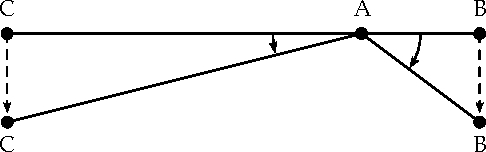
\includegraphics{efecto_distancia}
\decoRule
\caption[Efecto de distancia]{Efecto de distancia\protect\footnotemark.}
\label{fig:efecto_distancia}
\end{figure}

\footnotetext{Adaptación del esquema presentado por Mauve \cite{Mauve2001}.}

Este protocolo también aprovecha el \textit{efecto de distancia} para reducir el
alcance de las actualizaciones. En la figura \ref{fig:efecto_distancia} se
muestra el efecto de distancia. El nodo A se considera estático, y los nodos B
y C se mueven la misma distancia y en la misma dirección. No obstante, desde la
perpectiva del nodo A, el nodo B tuvo un movimiento más significativo que el
nodo C. Por esta razón, el nodo A requiere actualizaciones de la ubicación del
nodo B con más frecuencia que del nodo C.

En \cite{Haas1999}, se propone un servicio de localización llamado
\textit{Uniform Quorum Systems} (UQS)\footnote{Sistemas de \textit{quorum}
uniformes.}, en el que las actulizaciones de ubicación van dirigidas a un
subconjunto de los nodos, llamado \textit{quorum}, y las peticiones pueden
ser referidas a un \textit{quorum} potencialmente diferente. Cuando la
intersección entre dos \textit{quorums} diferentes no es vacía, se garantiza
que se encontrará un versión actualizada de la ubicación.

En el ejemplo de la figura \ref{fig:quorum}, los nodos 1-6 son seleccionados
para conformar el servicio de localización; este subconjunto de nodos se
denomina \textit{backbone virtual}. El nodo D envía su posición al nodo 6,
que es el nodo perteneciente el \textit{backbone} virtual más cercano. El nodo
6 selecciona el \textit{quorum} A, que contiene los nodos 1, 2 y 6, para
almacenar la actualización del nodo D. El nodo S envía una solicitud al nodo 4
para obtener la ubicación del nodo D. Este selecciona el \textit{quorum} B,
formado por los nodos 4, 5 y 6, para consultar la ubicación.

\begin{figure}[th]
\centering
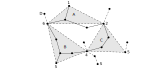
\includegraphics{quorum}
\decoRule
\caption[Ejemplo de \textit{quorum}]{Ejemplo de \textit{quorum}\protect\footnotemark.}
\label{fig:quorum}
\end{figure}

\footnotetext{Adaptación del esquema presentado por Mauve \cite{Mauve2001}.}

Otro servicio de localización es \textit{Grid Location Service}
(GLS)\footnote{Servicio de localización de cuadrícula.} \cite{Li2000}. En este
caso, la región donde se encuentra la red se divide de manera jerárquica en
cuadrados. Cuatro cuadrados de orden $n$ están contenidos dentro de un cuadrado
de orden $n+1$; cuatro cuadrados de orden $n+1$ están contenidos dentro de un
cuadrado de orden $n+2$, y así sucesivamente según se necesite.

El funcionamiento de GLS se muestra en la figura \ref{fig:gls}. Para determinar
cómo se almacena la posición de un nodo, se introduce el concepto de
\textit{nodo de ID cercano}, que se define de la siguiente manera: dado el
identificador de un nodo, su nodo de ID cercano el tiene el identificador mayor
más cercano al suyo entre los nodos que se encuentran dentro de un cuadrado. En
este ejemplo, el nodo 10 envía su ubicaión al nodo de ID cercano de cada uno de
los tres cuadrados circundantes de primer orden, que son los nodos 15, 18 y 73,
así como a todos los nodos que se encuentran dentro de su mismo cuadrado. En
cada uno de los tres cuadrados vecinos de segundo orden, también se selecciona
el nodo de ID cercano para compartirles su ubicación, que son los nodos 14, 25
y 29, como se muestra en la figura \ref{fig:gls1}. Este procedimiento se sigue
hasta cubrir toda el área de la red.

Si suponemos que el nodo 78 necesita conocer la ubiación del nodo 10, este debe
localizar y contactar a un nodo cercano que le pueda proporcionar ese dato. En
este caso, se trata del nodo 29. Así como el nodo 10 compartió su ubicación con
sus nodos de ID cercano, el nodo 29 compartió su ubicación con los nodos 36, 43
y 64. Hay que notar que, estos nodos automáticamente son nodos de ID cercano del
nodo 10 en su respectivo cuadrado, ya que también lo son del nodo 29. Por esto,
se puede rastrear el nodo 10 a través de una secuencia de identificadores de
nodos descendentes por cada uno de los cuadros de todos los órdenes. Es decir,
el nodo 78 obtiene del nodo 36 la ubicación del nodo 29 (orden 1), y obtiene
del nodo 29 la ubicación del nodo 10 (orden 2), como se observa en la figura
\ref{fig:gls2}.

\begin{figure}[th]
\centering

\begin{subfigure}[b]{\textwidth}
\centering
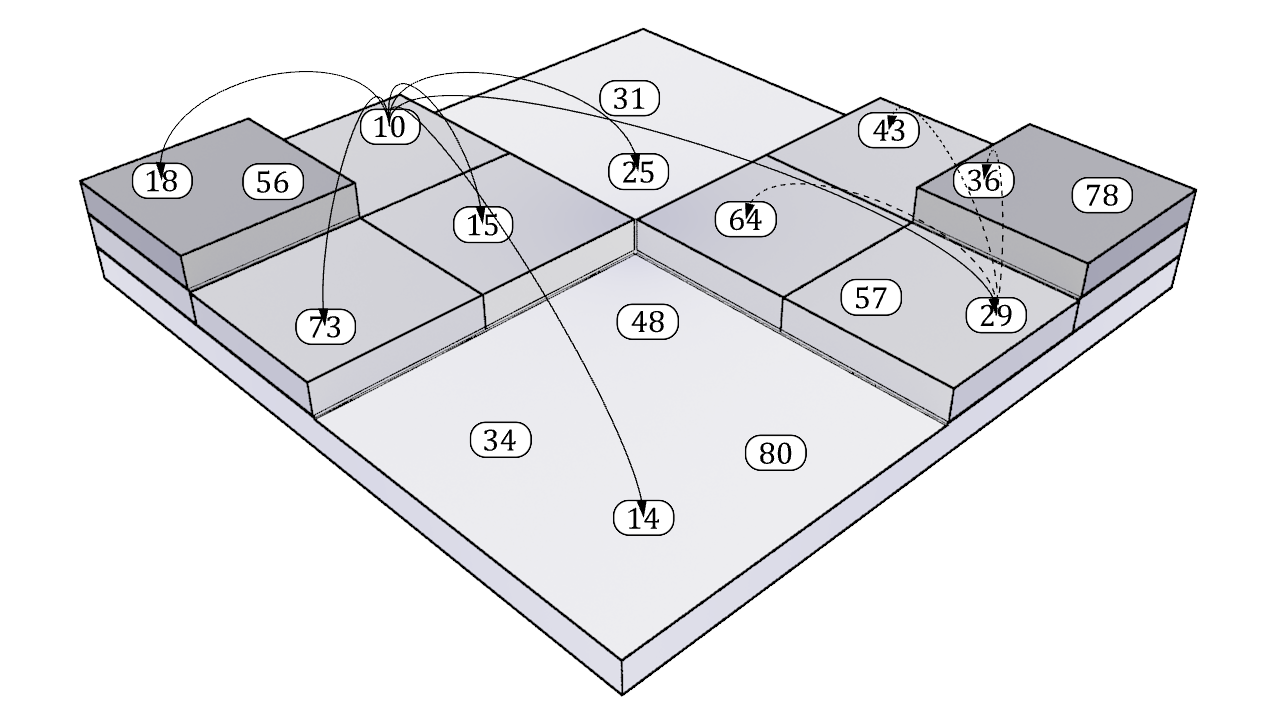
\includegraphics[scale=0.29]{gls1}
\caption{Almacenamiento de la ubicación de los nodos 10 y 29.}
\label{fig:gls1}
\end{subfigure}
\hfill
\begin{subfigure}[b]{\textwidth}
\centering
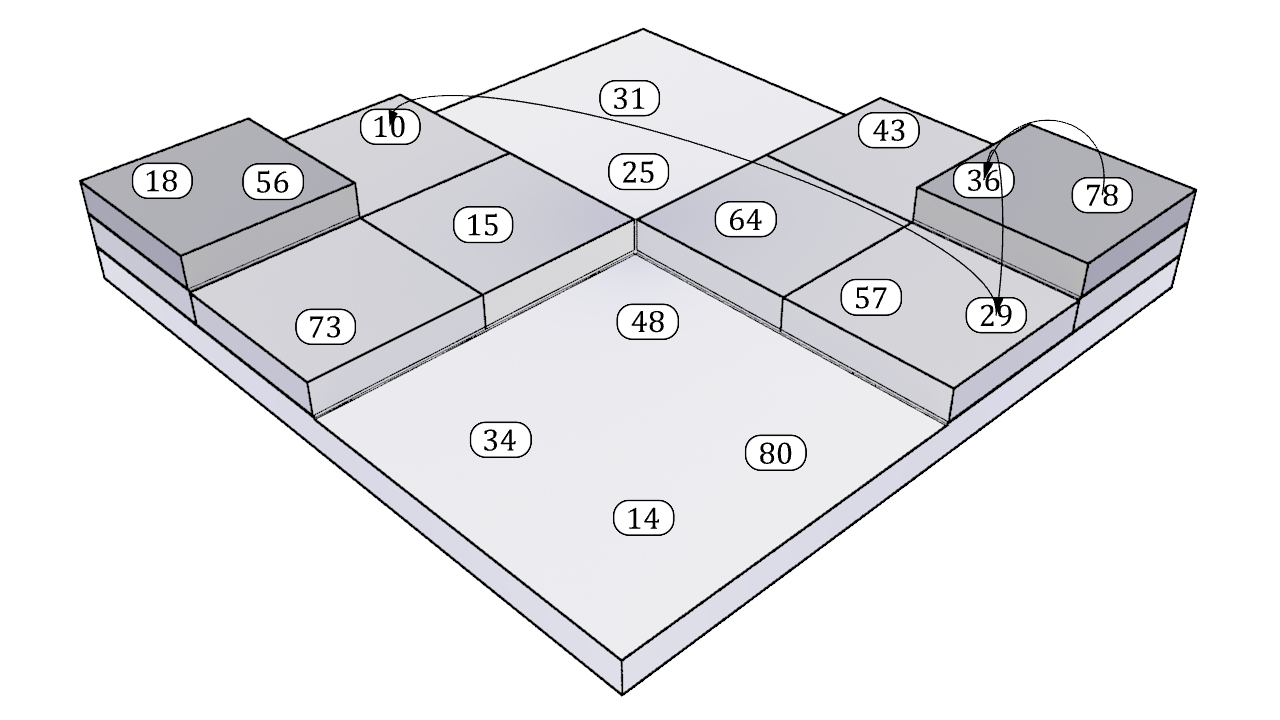
\includegraphics[scale=0.29]{gls2}
\caption{Descubrimiento de la ubicación del nodo 10 desde el nodo 78.}
\label{fig:gls2}
\end{subfigure}

\decoRule
\caption[Funcionamiento de GLS]{Funcionamiento de GLS\protect\footnotemark.}
\label{fig:gls}
\end{figure}

\footnotetext{Adaptación del esquema presentado por Mauve\cite{Mauve2001}.}

%-----------------------------------
%   ESTRATEGIAS DE RETRANSMISIÓN DE PAQUETES
%-----------------------------------
\subsection{Estrategias de retransmisión de paquetes}

\label{subsec:estrategias_de_retransmision_de_paquetes}

En esta sección se presentan algunos de los criterios que se consideran para la
retransmisión de paquetes a la hora de hacer el enrutamiento.

%-----------------------------------
%   RETRANSMISIÓN VORAZ
%-----------------------------------
\subsubsection{Retransmisión voraz}

\label{subsubsec:retransmision_voraz}

La retransmisión voraz consiste en considerar únicamente la información que se
tiene de manera inmediata para seleccionar hacia qué nodo retransmitir un
paquete. Ésta información, por lo general, es únicamente la ubicación del
destinatario y las de los vecinos que se encuentran dentro del área de cobertura. La
retransmisión se hace hacia alguno de los nodos que se encuentren más cerca del
destinatario, y este proceso se repite hasta que se llegue al destinatario.

\begin{figure}[th]
\centering
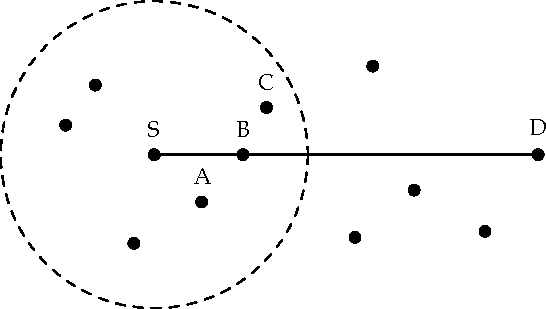
\includegraphics{retransmision_voraz}
\decoRule
\caption[Estrategias de retransmisión voraz]{Estrategias de retransmisión
voraz\protect\footnotemark.}
\label{fig:retransmision_voraz}
\end{figure}

\footnotetext{Adaptación del esquema presentado por Mauve\cite{Mauve2001}.}

Existen distintas maneras de seleccionar el siguiente salto. Estas se
ejemplifican en la figura \ref{fig:retransmision_voraz}, donde el nodo S es
el remitente y el nodo D es el destinatario. El círculo alrededor del nodo S
indica su radio máximo de transmisión. Uno de los criterios para seleccionar el
siguiente salto se seleccionar el vecino más cercano al destinatario. En el
ejemplo, este sería el nodo C. La idea es minimizar el número de saltos para
llegar al destino.

Otro método para seleccionar el siguiente salto es elegir el vecino más cercano
que se encuentre en la dirección del destinatario. En la figura
\ref{fig:retransmision_voraz}, este sería el nodo A. Este criterio es
conveniente si el nodo que retransmite es capaz de ajustar la potencia de la
transmisión, ya que se reduce la probabilidad de que existan colisiones con
otras transmisiones.

Otra regla que se puede seguir es seleccionar el vecino que esté más cercano a
la línea recta que une al remitente y al destinatario. En el ejemplo de la
figura \ref{fig:retransmision_voraz}, se trata del nodo B. El objetivo es
minimizar la distancia que viaja un paquete para llegar a su destino. También
es posible seleccionar aleatoriamente algún vecino que se encuentre más cerca
del destinatario. Esto reduce la precisión de la información requerida para
hacer la selección del siguiente nodo, además de que agiliza su selección, ya
que la cantidad de operaciones necesarias para esta operación es menor.

Por desgracia, la retransmisión voraz puede fallar cuando un nodo que va a
retransmitir un paquete está más cercano al destinatario que todos sus vecinos,
lo que se conoce como \textit{máximo local}. En este caso, no se podría
encontrar una ruta hacia el destinatario aunque exista al menos una. Esta
situación se ilustra en la figura \ref{fig:retransmision_voraz_falla}. En el
protocolo \textit{Greedy Perimeter Stateless Routing}
(GPSR)\footnote{Enrutamiento voraz y de perímetro sin estado.} propuesto por
Karp \textit{et al.} \cite{Karp2000}, cuando un paquete llega a un máximo
local, entra en un modo de recuperación cuyo criterio de retransmisión es
distinto al voraz, y regresa al modo voraz cuando llega a un nodo que está más
cercano al destinatario que el nodo donde entró al modo de recuperación.

\begin{figure}[th]
\centering
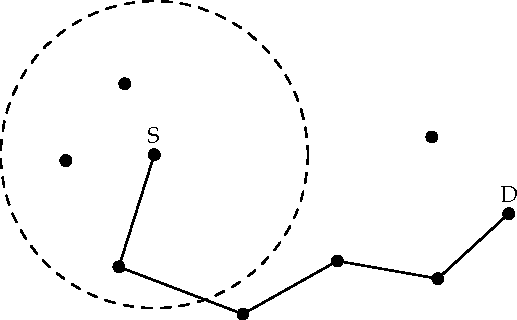
\includegraphics{retransmision_voraz_falla}
\decoRule
\caption[Falla en la retransmisión voraz]{Falla en la retransmisión
voraz\protect\footnotemark.}
\label{fig:retransmision_voraz_falla}
\end{figure}

\footnotetext{Adaptación del esquema presentado por Mauve\cite{Mauve2001}.}

El modo de recuperación del protocolo GPSR consiste en construir un subgrafo
plano con la ubicación de los vecinos y la del nodo que va a retransmitir el
paquete. La retransmisión se hace por el interior de las caras del subgrafo
usando la regla de la mano derecha. La figura \ref{fig:recuperacion_gpsr}
muestra cómo se usa el modo de recuperación para que un paquete llegue del nodo
S al nodo D. Se retransmite el paquete en la siguiente arista en el sentido
antihorario de la arista desde la que llegó. Cuando la arista tentativa de
retransmisión intersecta con la línea recta que une el remitente y el
destinatario, se verifica si esa intersección está más cerca del destinatario
que cualquier otra intersección encontrada anteriormente. Si este es el caso,
se cambia a la cara que está al otro lado de la arista tentativa, y se hace la
retransmisión por la siguiente arista en el sentido antihorario.

La cabecera del paquete contiene información para poder llevar a cabo el modo de
recuperacion, como la ubicación del nodo donde entró en este modo, la posición
de la última intersección que causó un cambio de cara, y la primera arista que
atravesó en la cara actual. Es por esto que cada nodo puede hacer la
retransmisión únicamente conociendo los vecinos que tiene dentro de su área de
cobertura. También se puede determinar si el destinatario está fuera de alcance,
que ocurre cuando el paquete pasa por la misma arista dos veces.

\begin{figure}[th]
\centering
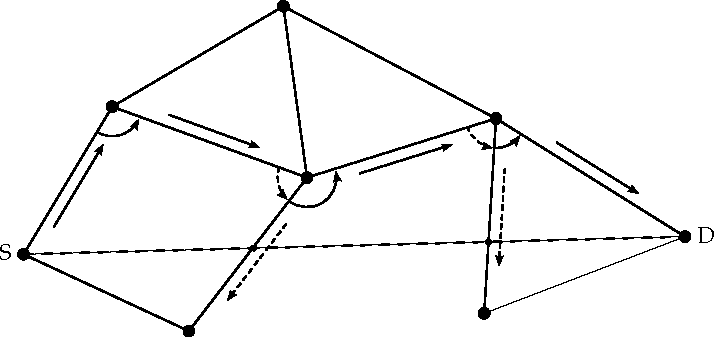
\includegraphics{recuperacion_gpsr}
\decoRule
\caption[Modo de recuperación de GPSR]{Modo de recuperación de
GPSR\protect\footnotemark.}
\label{fig:recuperacion_gpsr}
\end{figure}

\footnotetext{Adaptación del esquema presentado por Mauve\cite{Mauve2001}.}

%-----------------------------------
%   INUNDACIÓN DIRECCIONAL RESTRINGIDA
%-----------------------------------
\subsubsection{Inundación direccional restringida}

\label{subsubsec:inundacion_direccional_restringida}

El protoclo DREAM, discutido en la sección
\ref{subsec:servicios_de_localizacion}, usa esta técnica de retransmisión de
paquetes. En la figura \ref{fig:dream_region_esperada} se muestra el nodo S,
que quiere enviar un paquete al nodo D. El nodo S transmite el paquete a todos
sus vecinos que se encuentran en la dirección del nodo D. Para determinar esta
dirección, se calcula la región donde es probable que se encuentre el nodo D,
llamada \textit{región esperada}. Debido a que nada impide que el nodo D se
pueda mover en cualquier dirección, la región esperada es un círculo de radio
$v_{max}(t_1-t_0)$, donde $t_0$ es el tiempo en el que se registró la última
ubicación del nodo D, $t_1$ es el tiempo en el que se calcula la región
esperada, y $v_{max}$ es la velocidad máxima a la que se puede mover el nodo D.
El centro de este círculo es la ubicación del nodo D en el tiempo $t_0$.

\begin{figure}[th]
\centering
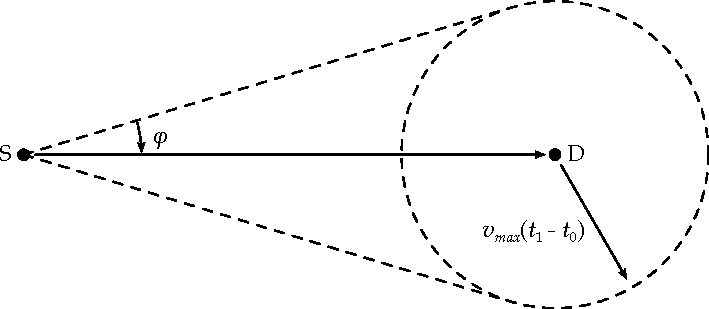
\includegraphics{dream_region_esperada}
\decoRule
\caption[Región esperada en el protocolo DREAM]{Región esperada en el protocolo
DREAM\protect\footnotemark.}
\label{fig:dream_region_esperada}
\end{figure}

\footnotetext{Adaptación del esquema presentado por Mauve\cite{Mauve2001}.}

Dada la región esperada, la dirección hacia el nodo D está delimitada por la
línea recta entre el nodo S y el nodo D y el ángulo $\varphi$. En otras
palabras, un nodo se encuentra en la dirección del nodo D si se encuentra
dentro del área delimitada por la región esperada y las dos líneas que empiezan
en el nodo S y son tangentes al círculo del perímetro de la región esperada. El
nodo S retransmite el paquete hacia sus vecinos que se encuentren en esa
dirección, y cada uno repite el proceso considerando su propia actualización de
la ubicación del nodo D. En caso de que no haya disponible un vecino que cumpla
con este criterio, se requiere un método de recuperación; sin embargo, este no
se especifica en el protocolo DREAM.

%-----------------------------------
%   ENRUTAMIENTO JERÁRQUICO
%-----------------------------------
\subsubsection{Enrutamiento jerárquico}

\label{subsubsec:enrutamiento_jerarquico}

Las redes de infraestructura fija pueden llegar a ser increíblemente complejas,
por lo que se organizan de manera jerárquica para lidiar con esta complejidad.
Por ejemplo, los enrutadores que forman el \textit{backbone} de la Internet se
organiza en \textit{Autonomous Systems} (ASs), o sistemas autónomos. El
enrutamiento de paquetes dentro del mismo AS se rige por un \textit{Interior
Gateway Protocol} (IGP)\footnote{Protocolo de puerta de enlace interior.}, como
el protocolo \textit{Open Shortest Path First} (OSPF)\footnote{Abrir el camino
más corto primero.} o \textit{Routing Information Protocol}
(RIP)\footnote{Protocolo de información de enrutamiento.}. Cuando un paquete
tiene que atravesar varios ASs, se utiliza un \textit{Interior Gateway Protocol}
(EGP)\footnote{Protocolo de puerta de enlace exterior.} al pasar de un AS a
otro; por ejemplo, \textit{Border Gateway Protocol} (BGP)\footnote{Protocolo
de puerta de enlace de frontera.}.
Esto facilita el enrutamiento a través de la Internet importantemente a pesar de
la enorme cantidad de dispositivos que la conforman. Por esta razón, es válido
preguntarse si el enrutamiento se puede beneficiar en las MANETs introduciendo
una estructura jerárquica.

En \cite{Blaevi2002}, Blaevi \textit{et al.} presentan el proyecto Terminode,
en el que se establece una jerarquía de dos niveles. El enrutamiento se hace
con un protocolo llamado \textit{Terminode Local Routing}
(TLR)\footnote{Enrutamiento local Terminode.} si el nodo de origen y el nodo de
destino están a pocos enlaces de distancia. TLR es un protocolo proactivo que
no usa las ubicaciones para seleccionar determinar las rutas. Cuando se trata
de distancias largas, se usa el protocolo \textit{Terminode Remote Routing}
(TRR)\footnote{Enrutamiento remoto Terminode.}, que usa el método voraz para
acercar el paquete al destinatario. Una vez que el paquete llega a una región
cercana al destinatario, TLR se encarga de que el paquete llegue al nodo
correspondiente. El funcionamiento del enrutamiento Terminode se muestra en la
figura \ref{fig:terminode}.

\begin{figure}[th]
\centering
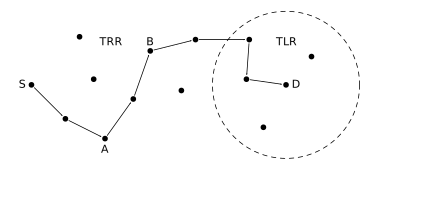
\includegraphics{terminode}
\decoRule
\caption[Enrutamiento Terminode]{Enrutamiento Terminode.}
\label{fig:terminode}
\end{figure}

Para prevenir que el protocolo TRR alcance un máximo local, el remitente incluye
una lista de ubicaciones por las que debe pasar el paquete. En la figura
\ref{fig:terminode}, se trata de los nodos A y B. Este método tiene cierta
similitud con la ruta de origen del protocolo DSR discutido en la sección
\ref{subsec:enrutamiento_reactivo}. Para conocer estas ubicaciones, el nodo
de origen solicita esta información a los nodos con los que tiene contacto
mediante TLR. Una vez que el nodo consigue esta información, debe verificar que
esta ruta de ubicaciones sigue vigente y si se puede optimizar.

%-----------------------------------
%   PROTOCOLOS DE ENRUTAMIENTO BASADOS EN LA POSICIÓN
%-----------------------------------
\subsection{Protocolos de enrutamiento basados en la posición para VANETs}

\label{subsec:protocolos_de_enrutamiento_basados_en_la_posicion_para_vanets}

Las características particulares de las VANETs introducen retos que no se
presentan en otros tipos de redes durante el proceso de enrutamiento. En esta
sección, se discuten algunos protocolos de enrutamiento especialmente diseñados
para lidiar con algunas de estas dificultades.

%-----------------------------------
%   GSR
%-----------------------------------
\subsubsection{GSR}

\label{subsubsec:gsr}

En \cite{Lochert2003}, Locher \textit{et al.} analizan las debilidades del
protocolo GPSR en un ambiente urbano, y proponen el protocolo
\textit{Geographic Source Routing} (GSR)\footnote{Enrutamiento de origen
geográfico.}. Este protocolo se apoya en un mapa de la ciudad para hacer el
enrutamiento basado en la posición.

Uno de los principales problemas del protocolo GPSR es que no considera la
existencia de obstáculos que deterioran la comunicación entre los nodos, como
los edificios en el ambiente de una VANET. Con el protocolo GSR, cuando un nodo
envía un paquete, usa el algoritmo de Dijkstra para calcular la ruta como una
secuencia de intersecciones de calles que el paquete debe atravesar para llegar
a su destino. Cuando un paquete viaja de una intersección a otra, se usa el
enfoque voraz para la retransmisión, ya que se asume que a lo largo de la calle
no existen obstáculos importante. Sin embargo, no incluye un método para
asegurar que a lo largo no se encuentre un máximo local.

GSR usa un servicio de localización simple llamado \textit{Reactive Location
Service} (RLS)\footnote{Servicio de localización reactivo.}. Cuando un nodo
necesita conocer la ubicación de otro, inunda la red con un mensaje de
solicitud. Si el nodo buscado recibe el mensaje, envía una respuesta con su
ubicación al nodo que hizo la solicitud. Este mecanismo incluye algunos
optimizaciones para evitar saturar toda la red con este tipo de solicitudes.

%-----------------------------------
%   SRPMT
%-----------------------------------
\subsubsection{SRPMT}

\label{subsubsec:srpmt}

El protocolo \textit{Street-centric Routing Protocol based on Microtopologies}
(SRPMT)\footnote{Protocolo de enrutamiento centrado en calles basado en
microtopologías.}, desarrollado por Zhang \textit{et al.} \cite{Zhang2016}
introduce el concepto de \textit{microtopología} (MT), que es un subconjunto de
toda la topología de la VANET. La MT comprende a los vehículos que se encuentran
a lo largo de una calle entre dos intersecciones consecutivas, y los enlaces
entre ellos, como se muestra en la figura \ref{fig:microtopologia}.

\begin{figure}[th]
\centering
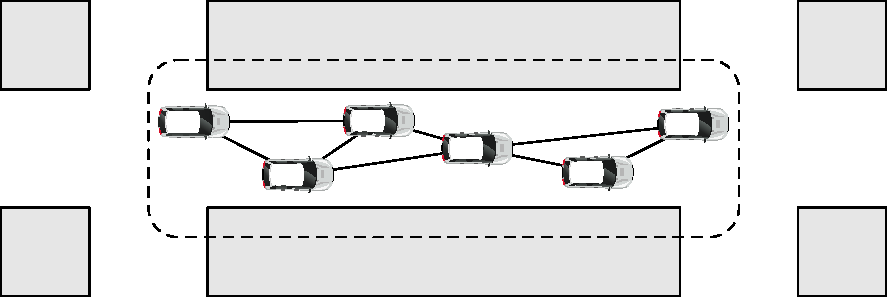
\includegraphics{microtopologia}
\decoRule
\caption[Microtopología]{Microtopología\protect\footnotemark.}
\label{fig:microtopologia}
\end{figure}

\footnotetext{Adaptación del esquema presentado por Zhang
\textit{et al.}\cite{Zhang2016}.}

Para llevar un paquete del nodo de origen al nodo de destino, la ruta puede
pasar por varias MTs. La estrategia de enrutamiento del protocolo SRPMT consiste
en dos pasos. El primero es determinar hacia qué MT se tiene que dirigir un
paquete una vez que llega al final de la MT que se encuentra atravesando. El
segundo paso es llevar el paquete del inicio de la MT hasta el final mediante
saltos por los nodos que la conforman. Cuando llega al último nodo de la MT,
este obtiene información de las MTs adyacentes y retransmite el paquete hacia
la que este nodo determine.

Este proceso se ilustra en la figura \ref{fig:ruta_microtopologias}, donde el
nodo S envía un paquete dirigido al nodo D. La microtopología $MT_{ij}$ comienza
en la intersección i y termina en la intersección j. Las flechas que se
encuentran dentro de la MT representan la dirección del avance del paquete a lo
largo de la MT. Las flechas que van de una MT a otra representan la selección
de la siguiente MT en la ruta.

\begin{figure}[th]
\centering
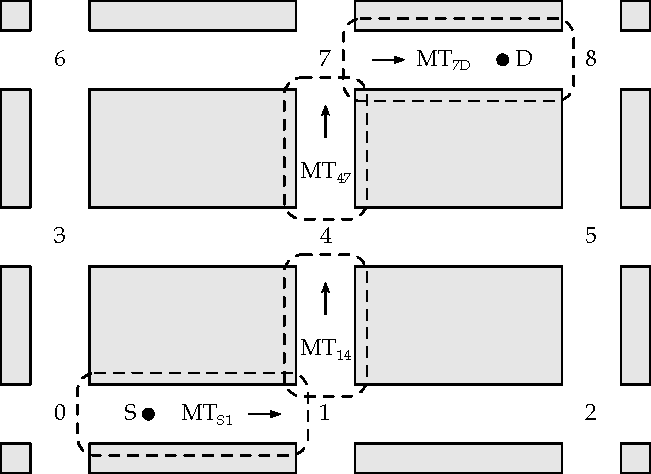
\includegraphics{ruta_microtopologias}
\decoRule
\caption[Ruta a lo largo de varias microtopologías]{Ruta a lo largo de
varias microtopologías\protect\footnotemark.}
\label{fig:ruta_microtopologias}
\end{figure}

\footnotetext{Adaptación del esquema presentado por Zhang
\textit{et al.}\cite{Zhang2016}.}

A pesar de que una MT puede modificarse constantemente según la movilidad de los
autos, la dirección hacia la que se tiene que mover el paquete es fija. Esto
significa que criterio para la retransmisión es que el paquete avance hacia el
extremo de la MT. Existen dos factores principales que afectan el desempeño de
una MT. El primero es el desempeño del enlace, que incluye la tasa de éxito de
transmisión de paquetes, y la demora en la entrega de paquetes. El otro factor
determinante es la estrategia de enrutamiento interna de la MT.

%-----------------------------------
%   MM-GPSR
%-----------------------------------
\subsubsection{MM-GPSR}

\label{subsubsec:mm_gpsr}

El protocolo GPSR, presentado en la sección \ref{subsubsec:retransmision_voraz},
selecciona como siguiente salto el nodo más cercano al destinatario. El
principal problema es que, mientras más cercano esté un nodo del destinatario,
más lejos se encuentra del nodo que debe hacer la retransmisión del paquete.
Por esto, existe la posibilidad de que el nodo seleccionado quede fuera del área
de transmisión antes de recibir la transmisión correctamente. Esta situación se
puede presentar más fácilmente en una VANET que en otros tipos de redes
\textit{ad hoc}, debido a que el movimiento relativo entre los vehículos es muy
rápido, y pueden cambiar de dirección abrúptamente y perder el enlace de
comunicación.

Es por esto que Yang \textit{et al.} proponen el protocolo
\textit{Maxduration-Minangle GPSR} (MM-GPSR)\footnote{Enrutamiento voraz y de
perímetro sin estado de másxima duración y ángulo mínimo.} \cite{Yang2018},
cuya principal característica es la modificación del criterio voraz de
selección del siguiente salto que se usa en GPSR. En la figura \ref{fig:mmgpsr}
se muestra la regla voraz del protocolo MM-GPSR, en el que el nodo S quiere
transmitir un paquete al nodo D. Primero, se determina el vecino más cercano al
nodo D, que es el nodo B en el ejemplo. Después, se obtiene la distancia
$d_{BD}$ entre los nodos B y D, y la distancia $d_{SB}$ entre los nodos S y B.
Posteriormente, se calcula $d_{max}$ con la ecuación \ref{eq:1}. Con estos
datos, se consideran dos círculos, el primero con centro en el nodo S y cuyo
radio es la distancia máxima de transmisión de este, y el segundo con centro en
el nodo D y con radio $d_{max}$. La región delimitada por la intersección de
ambos círculos se denomina $Q$. Cada nodo dentro de $Q$ se encuentra cerca del
nodo D, y está dentro del radio de comunicación del nodo S, por lo que es
apropiado para ser seleccionado para la retransmisión.

\begin{equation}
\label{eq:1}
d_{max} = d_{BD} + \lambda d_{SB}
\end{equation}

\begin{figure}[th]
\centering
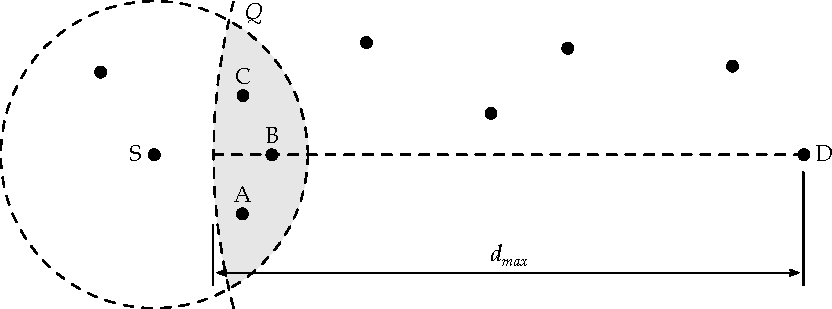
\includegraphics{mmgpsr}
\decoRule
\caption[Enrutamiento voraz en el protocolo MM-GPSR]{Enrutamiento voraz en el
protocolo MM-GPSR\protect\footnotemark.}
\label{fig:mmgpsr}
\end{figure}

\footnotetext{Adaptación del esquema presentado por Yang \textit{et
al.}\cite{Yang2018}.}

En la ecuación \ref{eq:1}, $\lambda$ puede variar desde 0 hasta 1. Si $\lambda$ se
acerca a 1, el área de $Q$ se hace más grande, y los vecinos más cercanos al nodo S
tienen oportunidad de ser seleccionados como siguiente salto, pero la cantidad
de saltos en la ruta incrementa. Si $\lambda$ se hacerca a 0, el área de $Q$ se
hace más pequeña, y los vecinos más lejanos al nodo S tienen más oportunidad
de ser seleccionados, por lo que la estabilidad del enlace puede empeorar
y la probabilidad de que se pierda el paquete aumenta.

Para seleccionar el siguiente salto, se considera la duración acumulada del
enlace de comunicación del nodo S con sus vecinos. Este dato se calcula con la
ecuación \ref{eq:2}, donde $T_{i-1}$ es la duración acumulada anterior del
enlace, $t_i$ es el tiempo de recepción de un mensaje \textit{hola}, y $t_{i-1}$
es el tiempo de recepción del mensaje \textit{hola} anterior. Las condiciones
iniciales son $T_1 = 0$ y $t_1$ es el tiempo en el que se recibe el primer
mensaje \textit{hola}. Al comparar el valor de $T_i$ para los nodos A, B y C,
el nodo con el máximo valor de $T_i$ es el que se selecciona como siguiente
salto, ya que su enlace con el nodo S es el que tiene el mejor historial de
estabilidad.

\begin{equation}
\label{eq:2}
T_i = T_{i-1} + t_i - t_{i-1}
\end{equation}

%-----------------------------------
%   VBRP
%-----------------------------------
\subsubsection{VBRP}

\label{subsubsec:vbpr}

Ji \textit{et al.} desarrollaron el protocolo \textit{Virtual Backbone-based
Routing Protocol} (VBRP)\footnote{Protocolo de enrutamiento basado en
\textit{backbone} virtual.} \cite{Ji2019}, en el que cada nodo puede ser de dos
tipos: normal o \textit{backbone}. Los nodos \textit{backbone} son las únicos
que partiipan en el enrutamiento, mientras los nodos normales pueden transmitir
y recibir paquetes a través de los nodos \textit{backbone}. La idea de dejar
fuera del enrutamiento a ciertos nodos es no saturar el canal de comunicación
para reducir las demoras por contenciones y prevenir las colisiones entre las
transmisiones. Para seleccionar los nodos \textit{backcone}, se define una
métrica llamada \textit{Stability Index} (SI), o índice de estabilidad. El SI
se obtiene a partir de dos parámetros, que son la estabilidad del enlace de
comunicación y la movilidad relativa entre los nodos. Los nodos con mayor SI se
seleccionan como nodos \textit{backbone}.

El funcionamiento general del protocolo VBPR se muestra en la figura
\ref{fig:vbpr}. El nodo S envía un paquete dirigido al nodo D, así que lo
transmite a un nodo \textit{backbone}, y este lo retransmite al siguiente nodo
\textit{backbone} que se encuentre adelante en el camino. En este protocolo
también se consideran dispositivos fijos llamadas \textit{Road Side Units}
(RSUs), o unidades laterales del camino, que toma las decisiones de
enrutamiento en las intersecciones.

\begin{figure}[th]
\centering
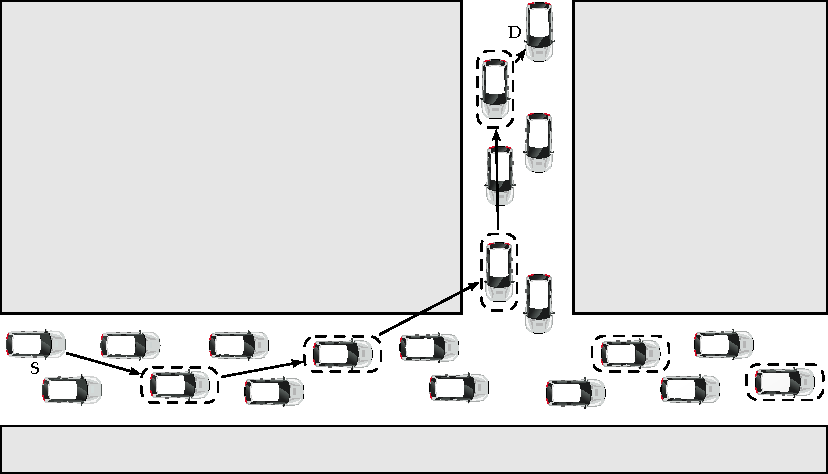
\includegraphics{vbpr}
\decoRule
\caption[Funcionamiento del protocolo VBRP]{Funcionamiento del protocolo VBRP\protect\footnotemark.}
\label{fig:vbpr}
\end{figure}

\footnotetext{Adaptación del esquema presentado por Ji
\textit{et al.}\cite{Ji2019}.}
